
\documentclass[12pt]{amsart}
\usepackage{listings}
\usepackage{color}
\usepackage{graphicx}

\definecolor{dkgreen}{rgb}{0,0.6,0}
\definecolor{gray}{rgb}{0.5,0.5,0.5}
\definecolor{mauve}{rgb}{0.58,0,0.82}

\lstset{frame=tb,
  language=Python,
  aboveskip=3mm,
  belowskip=3mm,
  showstringspaces=false,
  columns=flexible,
  basicstyle={\small\ttfamily},
  numbers=none,
  numberstyle=\tiny\color{gray},
  keywordstyle=\color{blue},
  commentstyle=\color{dkgreen},
  stringstyle=\color{mauve},
  breaklines=true,
  breakatwhitespace=true,
  tabsize=3
}
\title{NLP_HW3}
\author{Xuan Wang}
\date{} % delete this line to display the current date

%%% BEGIN DOCUMENT
\begin{document}


\section{Question 0}
For the maze, define a maze class, use \emph{numpy} external library to generate a 2-d 101*101 int array representing the maze. Then use \emph{networkx} library to convert the maze into an undirected graph by adding edges for each pair of adjacency nodes, use \emph{dfs\_preorder\_nodes()} method to find a traverse list by DFS, for each visited node make it blocked of 30\% chance
\begin{lstlisting}
self.array = np.zeros((m,n))
traverselist = list(nx.dfs_preorder_nodes(self.graph,(0,0)))
p_list = [1,1,1,0,0,0,0,0,0,0]
traverselist = self.DFS()
for i in traverselist:
	self.array[i[0],i[1]] = random.choice(p_list)
\end{lstlisting}
%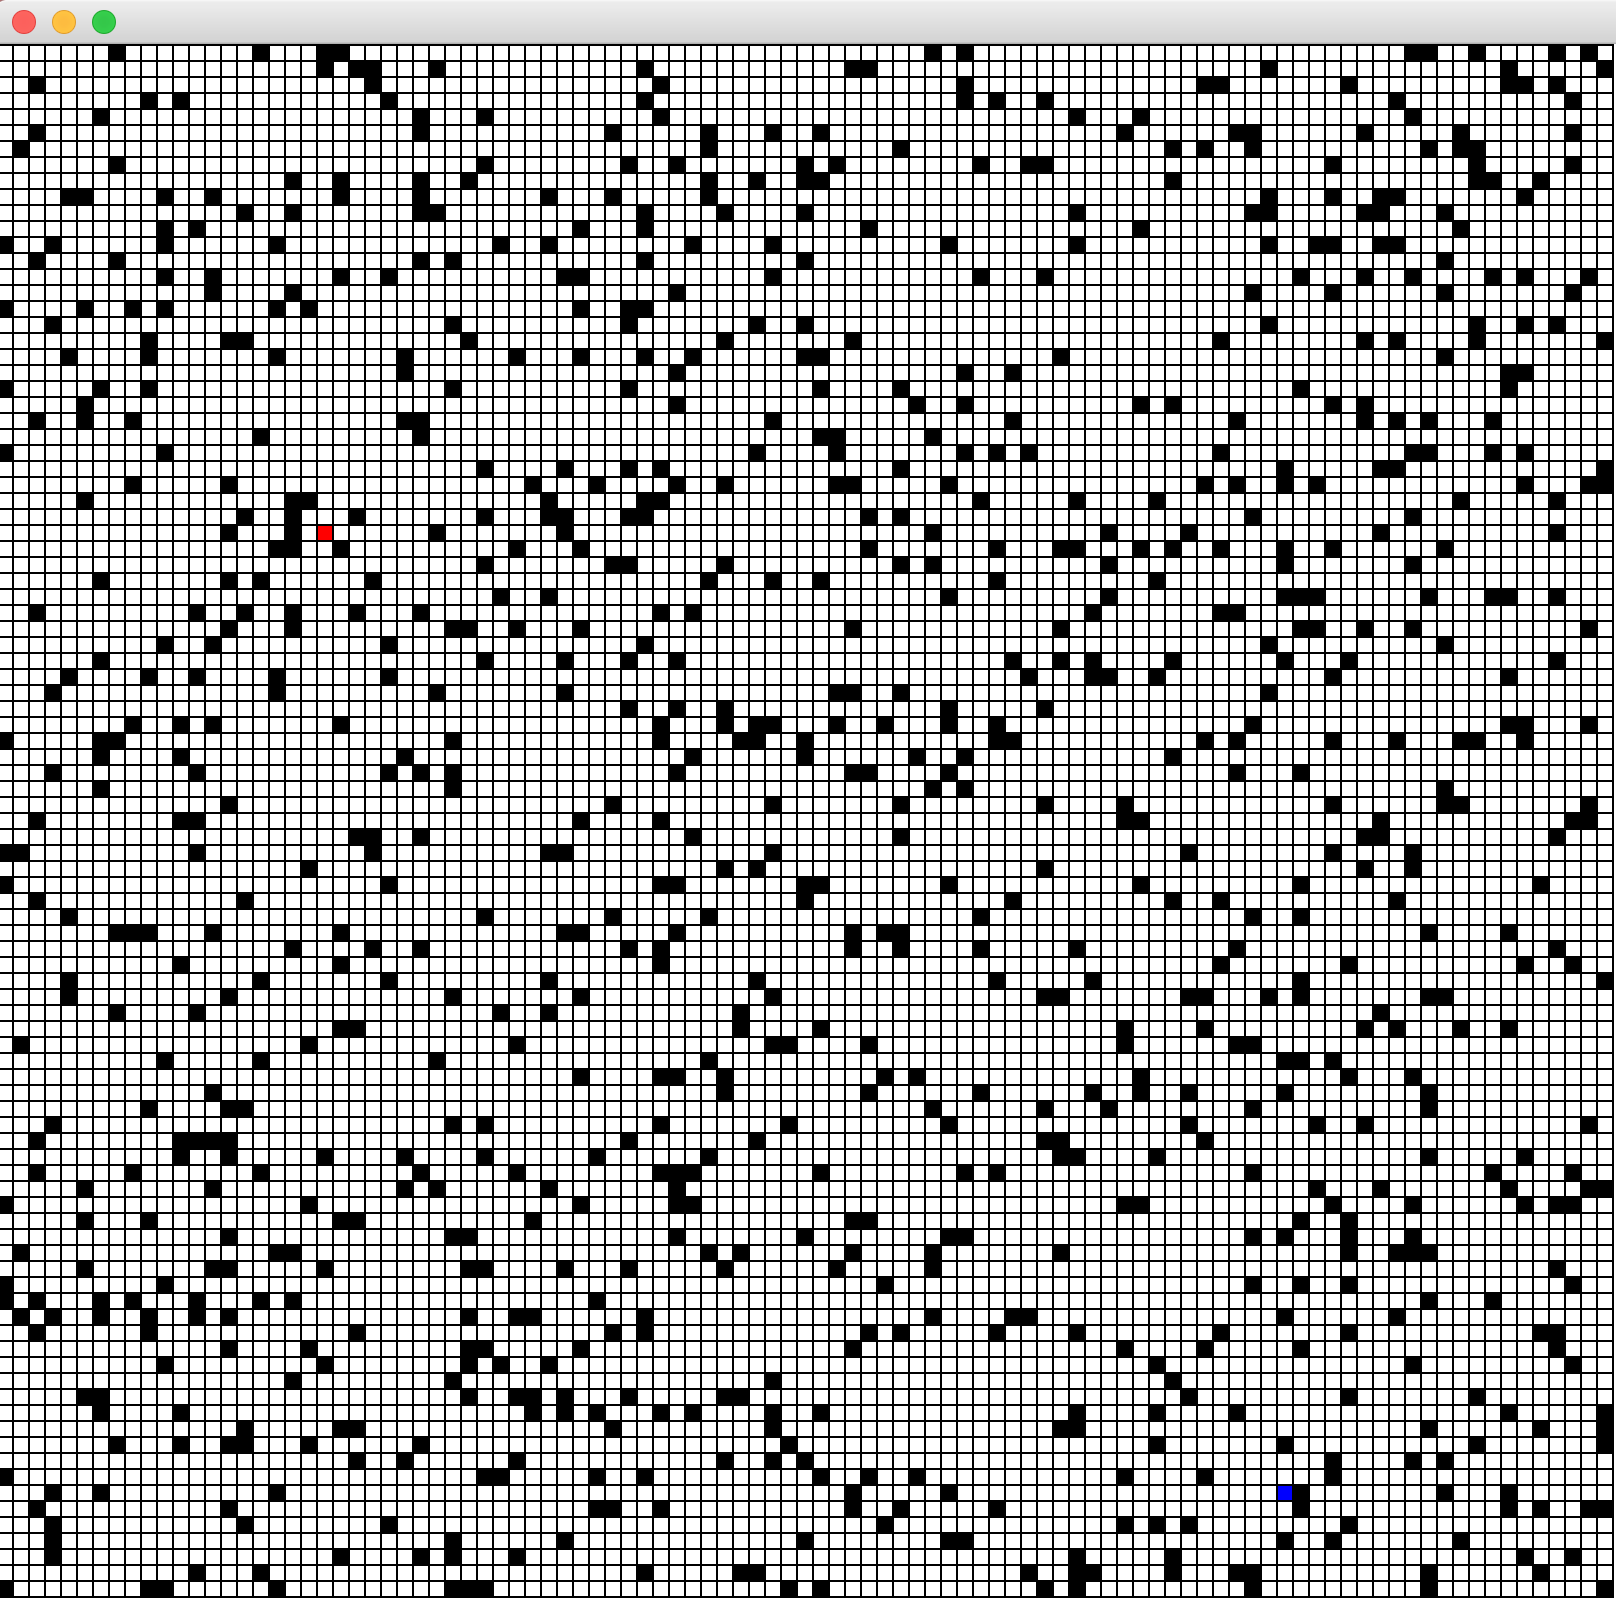
\includegraphics[width=1\linewidth]{maze.png}

\section{Part 1}
(a)While the initial agent explored three cells next to it which is unblocked, the three cells have same \emph{g-values} 1, different \emph{h-values}. Base on Manhhatan distance, the right one cell has the samllest \emph{g-value} 2, so it has the smallest \emph{f-value} 3, so the right one will be expanded first.

(b)Since the algorithm finds cell with minimum f value from open list and add it to close list, if open list is running to empty without found a end node, that means no more unvisited cells can be expanded and there is no path from start node to target node. It is always possible to find a path or find it impossible before all unblocked cells are added into close list, so the result can be found in finite time. The worst case is that the agent finds block and change path at each unblocked cell, and for each cell the agent goes through all possible unblocked cells and find a dead end. So the bound of agent moves is the number of unblocked cells squared.

\section{Part 2}
smaller g

larger g
\section{Part 3}
\section{Part 4}
The definition of Manhattan distance: The distance between two points measured along axes at right angles. If the agent only moves in four compass directions, it will only move along the axes we built, it assures that the Manhattan distances are consistent.

(OFFICIAL ANSWER)Adaptive A* solves a series of similar but not necessar- ily identical search problems. However, it is important that the h-values remain consistent with respect to the goal state from search problem to search problem. The following changes can occur from search problem to search problem:
? The start state changes. In this case, Adaptive A* does not need to do anything since the h-values remain consistent with respect to the goal state.
? The goal state changes. In this case, Adaptive A* needs to correct the h-values. Assume that the goal state changes from sgoal to s?goal. Adaptive A* then updates (= overwrites) the h-values of all states s by assigning
h(s) := max(H (s, s?goal ), h(s) ? h(s?goal )). (2)
The updated h-values are consistent with respect to the new goal state [9]. However, they are poten- tially less informed than the immediately preceeding h-values. Taking the maximum of h(s) ? h(s?goal) and theuser-suppliedH-valueH(s,s?goal)withrespectto the new goal state ensures that the h-values used by Adaptive A* dominate the user-supplied H-values with respect to the new goal state at least weakly.
? At least one action cost changes. If no action cost decreases, Adaptive A* does not need to do anything since the h-values remain consistent with respect to the goal state. This is easy to see. Let c denote the orig- inal action costs and c? the new action costs after the changes. Then, h(s) ? c(s, a) + h(succ(s, a)) for s ?
\section{Part 5}
\section{Part 6}
The tree pointer can be 
\end{document}